    \begin{algorithm}[!t]
        \centering
        \caption{Unifying the character font style}
        \label{alg:unify_font_style}
        \begin{algorithmic}[1]
            \REQUIRE~~\\
                $CI$: Captcha Image  \\
                $numChar$: The number of characters on Captchas\\
            \ENSURE~~\\
                $UC$: Captcha with the same font style \\
            \STATE $grayCI \leftarrow getBinaryImage(CI)$ \\
            \STATE $positions[] \leftarrow getHollowPositions(grayCI)$ \\
            \STATE $LEN \leftarrow getPositonsLen(positions[], numChar)$ \\
            \STATE $meanThick \leftarrow getMeanCharThick(CI, positions[])$ \\
            \FOR{$i=1:LEN$}
                \STATE $cFI \leftarrow FillRedColor(CI, positions[i])$ \\
                \STATE $cCI \leftarrow ChangeFillColor(cFI, positions[i])$ \\
                \STATE $charThick \leftarrow getCharThick(cCI, positions[i])$ \\
                \IF{$charThick>meanThick$}
                    \STATE $UC=cropChar(cCI, positions[i], meanThick)$ \\
                \ENDIF
            \ENDFOR
        \end{algorithmic}
    \end{algorithm}
\section{Implementation Details}

\subsection{Captcha Preprocessing}
Given some current text-based Captchas mainly consist of both solid character and hollow character (see Figure~\ref{fig:text-based captchas} (j) and (k)), the first step of our attack is to unify the different font styles to a fixed style. Here we aims to fill the hollow character with solid core due to the following two reasons:
(1) the hollow character can be easily transformed to the solid one but not the opposite.
(2) the solid character can be extracted more stable features than hollow character at the following step according to our preliminary experiments.

To do so, we first convert the colorful image to black-and-white using the standard threshold selection method proposed by Otsu~\cite{Ostu1979A}\footnote{Note that we only use the binarized image to locate the position of the hollow part of the character other than furthering processing.}.
Then the Color Filling Segmentation (CFS)~\cite{Yan2008A} is used to fill the hollow character with the red color (see Figure~\ref{fig:fill_color} (b)). Next, the color-filled image should be convert to color-coincident image by changing the red filled area to the original character color (see Figure~\ref{fig:fill_color} (c)). At last, the thick filled characters on the color-coincident image need to be cropped as the original character (see Figure~\ref{fig:fill_color} (d)).

Our method for unifying the character font style is described in Algorithm~\ref{alg:unify_font_style}.
The input to the algorithm is the original Captcha image with different font styles and the number of characters on this Captcha, and the output of the algorithm is the Captcha with solid characters. To locate the hollow characters, we first convert the colorful original image to binarized image (line 1). According to the binarized image, we can get the positions of the each hollow characters on the colorful Captcha image (line 2) because the size of colorful image is the same as the binarized image. For each hollow character, we use CFS method described above to fill it with red color (line 6) and then replace the red filled color with the character color to get the color-coincident image (line 7). Finally, we crop the filled character on the color-coincident image to unify the font style of characters (line 10).

\subsection{Generate Regular Captcha}
After unifying the character font style, we need to generate regular Captchas for better recognizing. We achieve this by employing an image-to-image translation algorithm called Pix2Pix~\cite{Pix2PixCode}. This algorithm automatically translate the image from the original style to the target style. In our case, the images to be translated are the Captchas with complex noisy background, overlapping and distorted characters (original style). These are supplied to the algorithm by a Captcha generator developed using a simple script (Section~\ref{section: Captcha_generator}). The algorithm tries to generate regular Captcha with appropriate character spacing and clean background (target style).

In order to generate regular Captcha, we propose the hierarchical methods that employ a variant approach of \emph{Pix2Pix} to complete the progressive tasks.
These hierarchical methods share the same methodology of the variant algorithm.
The main differences of these hierarchical approaches are the input and output images. The inputs of the first steps are the images with complex background, overlapping and distorted characters.
These inputting images are eliminated the complex background by the variant approach which outputs the Captcha images with white background, overlapping and distorted characters.
According to the outputs, the second step is to expand the space between the adjacent overlapping characters using the same variant method, and produces the Captcha images only with distorted characters.
Finally, the distorted characters are translated to the regular ones using the variant method.

\noindent \textbf{Hierarchical Methods.} The hierarchical methods are comprised of three sequenced models, and they can respectively achieve the tasks of removing complex background, expanding space between adjacent overlapping characters and translating the distorted Captcha to a regular one. The sequenced models share the same translation model.
The key part of the translation model is a variant of \emph{Pix2Pix}, which consists of a image generator and discriminator. They are competing with each other until reach Nash equilibrium when training processing (Section~\ref{section: GANs}).

In our case of removing background, the inputting data are the image pairs including the Captcha images with complex background and the images with white background.
The goal is to train a generative model that can translate the Captcha image with complex background to the images with white background.
During training, the image generator produces the fake image that similar to the image with white background by randomly add the noisy points to it. The fake image and the image with complex background compose an image pair.
For the composed image pair, the discriminator learns to classify between the real and fake pairs. This competing process will be terminated until the discriminator cannot classify the image pairs.
Unlike the \emph{Pix2Pix}, we use the L2 distance to figure out the loss of the generator as L2 loss can capturing the overall structure of the Captcha image, which contribute to removing the background.
\begin{equation}\label{equation: L2_loss}
    \mathcal{L}_{L2}(Gen) = \mathbb{E}_{x,y \epsilon C_{O}, z \epsilon N_{O}} \|y - Gen(x, z)\|_{2}
\end{equation}

Where $x$ is the Captcha image with white background, $y$ is the image with complex background and $z$ is the fake image with the noisy points.

\begin{figure}[!t]
  \centering
  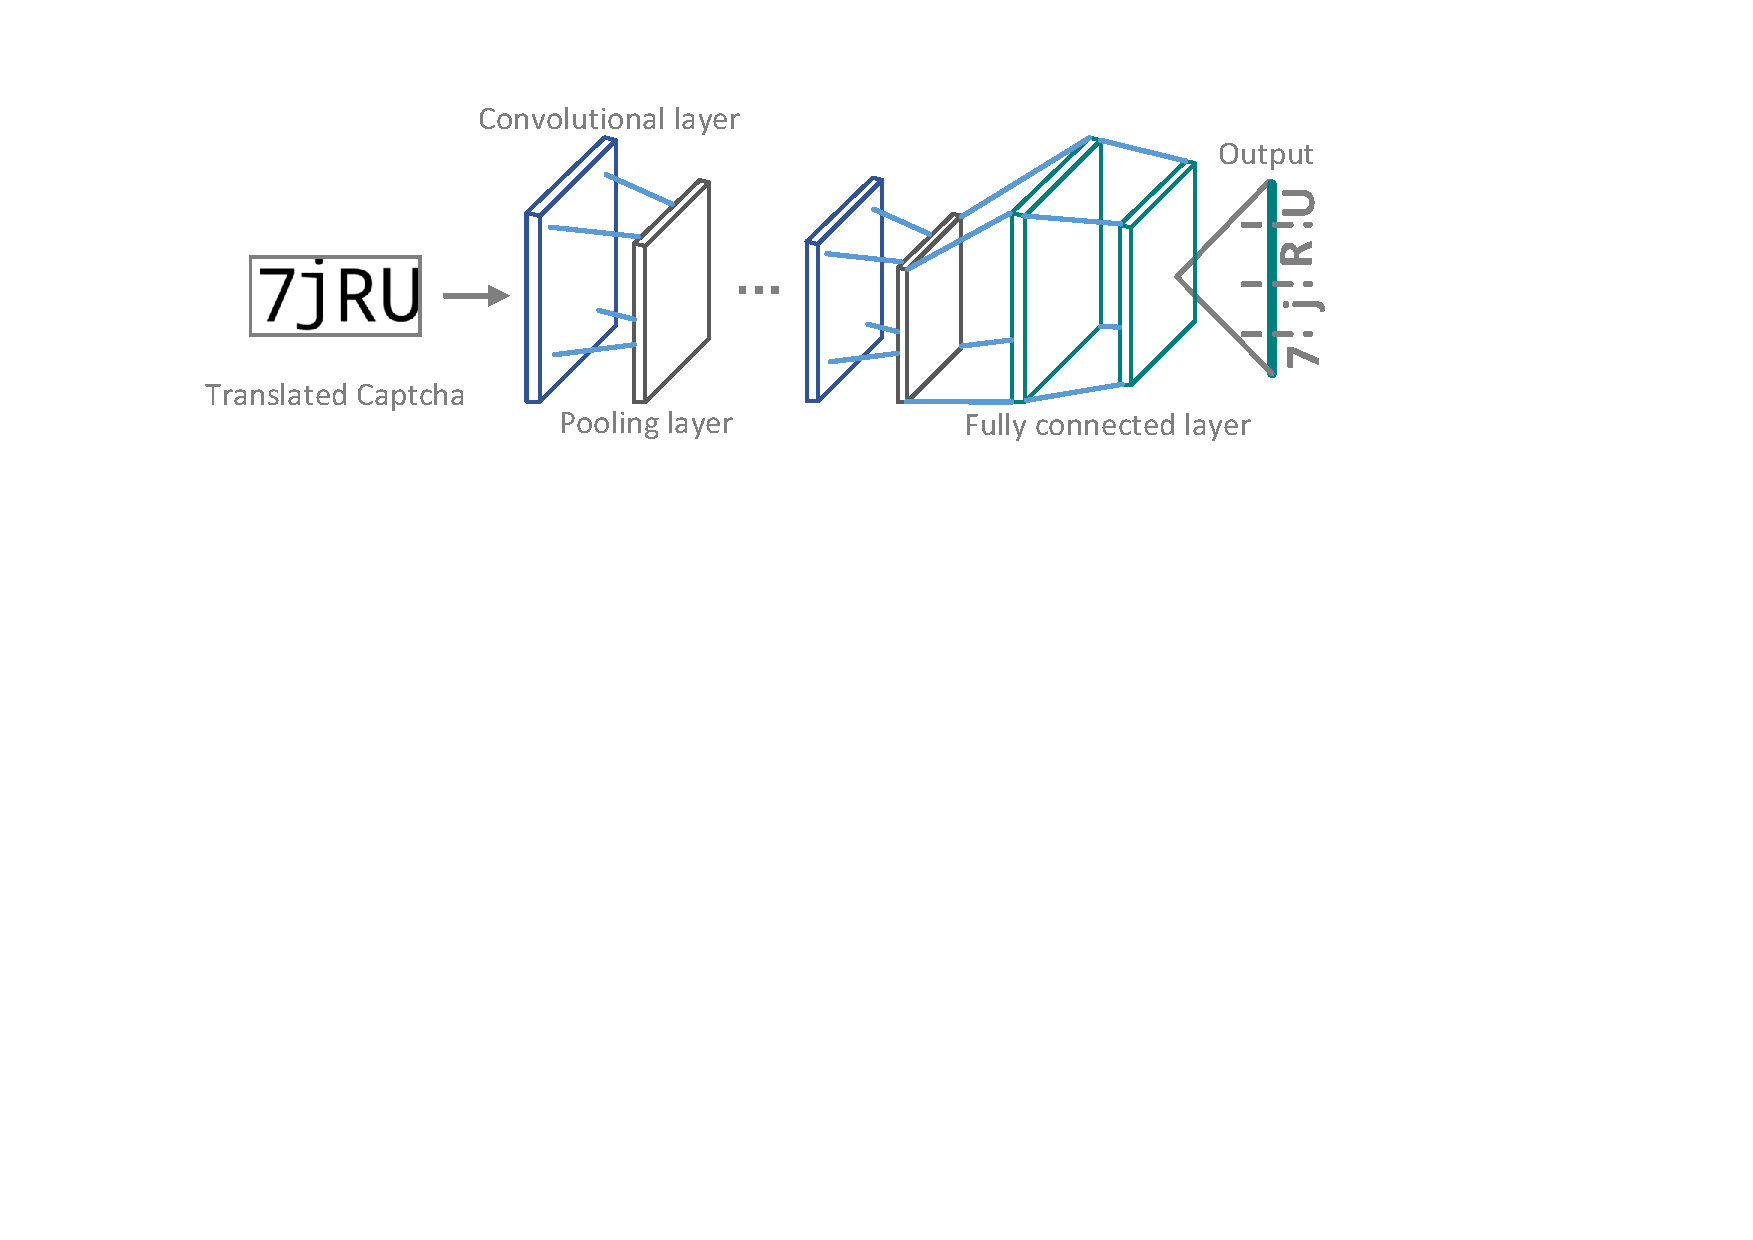
\includegraphics[width=0.45\textwidth]{fig/cnn_model.pdf}
  \caption{CNN recognition engine. The input of the recognition recognize is the regular Captcha image, and it output the text of the Captcha image.}
  \label{fig: cnn_model}
\end{figure}

\subsection{Identify Captcha}
In this step, we use a rudimentary CNN framework, \emph{LeNet-5}~\cite{Lecun1998Gradient}, as our recognition engine, to identify the text of the translated Captcha image.
The initial \emph{Lenet-5} was compromised of three convolutional layers, two pooling layers and followed by two fully connected layers.
The convolutional layer extracts the features using a number of filters that are trained during training process. The pooling layer aggregates the features extracted from the convolutional layer for extracting more representative features meanwhile reducing the amount of calculation. The fully connected layer classify the extracted features into target categories. The appropriate number of network layers determines the quality of the extracted features as proper number of layers will extract more representative features.

Unlike the \emph{LeNet-5}, the goal of our recognition engine is to recognize the text of Captchas on the whole, which is more difficult than recognition a single character done by \emph{LeNet-5}. This is because recognizing more characters need to extract more complex and abstract features.
To do so, we redesign the \emph{LeNet-5} and adding another two convolution layers and another three pooling layers.
Figure~\ref{fig: cnn_model} depicts the framework of our recognition engine. Generally, it consists of five convolution layers, five pooling layers and followed by two fully connected layers. Each convolution layer is followed by a pooling layer.

To extract more representative features, each convolutional layer uses a convolution filter of $3 \times 3$ and each pooling layer employs the max-pooling value. Other parameters are the same as the \emph{LeNet-5}.











